\documentclass[tikz,border=2pt]{standalone}
\usepackage{amsmath,amssymb}
\usepackage{tikz}
\usetikzlibrary{arrows.meta}

\begin{document}
% The incumbent is the best integer-feasible solution found so far; it only improves over
% time and its value L is the yardstick for pruning.
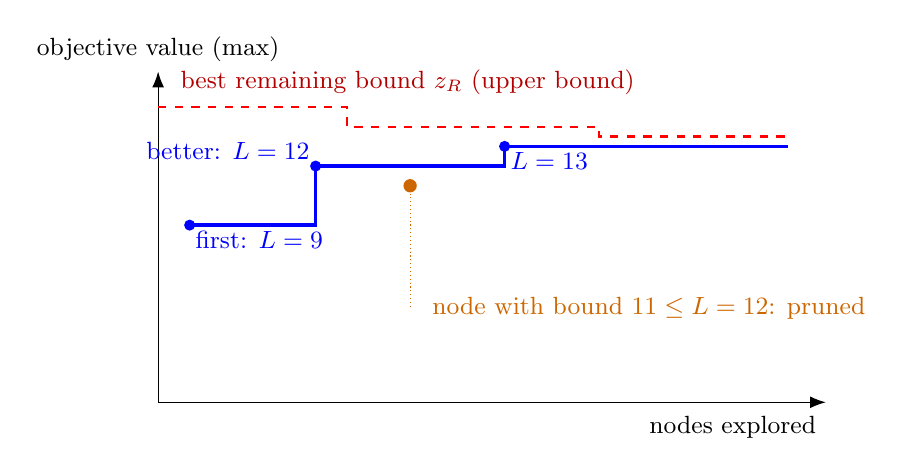
\begin{tikzpicture}[x=0.8cm, every node/.style={font=\small}, >={Latex[length=2mm]}]
	\draw[->] (0,0) -- (10.6,0);
	\node[anchor=north east] at (10.6,-0.05) {nodes explored};
	\draw[->] (0,0) -- (0,4.2) node[above] {objective value (max)};
    % A single vertical scale for all objective values and bounds: height = value / 4.
    \def\objscale{0.25}
    \draw[blue, very thick] (0.5,{\objscale*9}) -- (2.5,{\objscale*9}) -- (2.5,{\objscale*12}) -- (5.5,{\objscale*12}) -- (5.5,{\objscale*13}) -- (10,{\objscale*13});
    \fill[blue] (0.5,{\objscale*9}) circle (2pt) node[below right, inner sep=2pt] {first: $L=9$};
    \fill[blue] (2.5,{\objscale*12}) circle (2pt) node[above left, inner sep=2pt] {better: $L=12$};
    \fill[blue] (5.5,{\objscale*13}) circle (2pt) node[below right, inner sep=2pt] {$L=13$};
    \draw[red, dashed, thick] (0,{\objscale*15}) -- (3,{\objscale*15}) -- (3,{\objscale*14}) -- (7,{\objscale*14}) -- (7,{\objscale*13.5}) -- (10,{\objscale*13.5});
    \node[red!70!black, anchor=south west] at (0.2,3.78) {best remaining bound $z_R$ (upper bound)};
    \fill[orange!80!black] (4,{\objscale*11}) circle (2.4pt);
    \draw[orange!80!black, densely dotted] (4,{\objscale*11}) -- (4,1.2);
    \node[orange!80!black, anchor=west] at (4.2,1.2) {node with bound $11\le L=12$: pruned};
	\end{tikzpicture}
\end{document}
